\documentclass{article}
\usepackage{amsmath}
\usepackage{graphicx}
\usepackage{hyperref}
\usepackage{tikz}
\usetikzlibrary{arrows.meta, positioning, shapes.geometric}

\begin{document}

\begin{figure}[h]
    \centering
    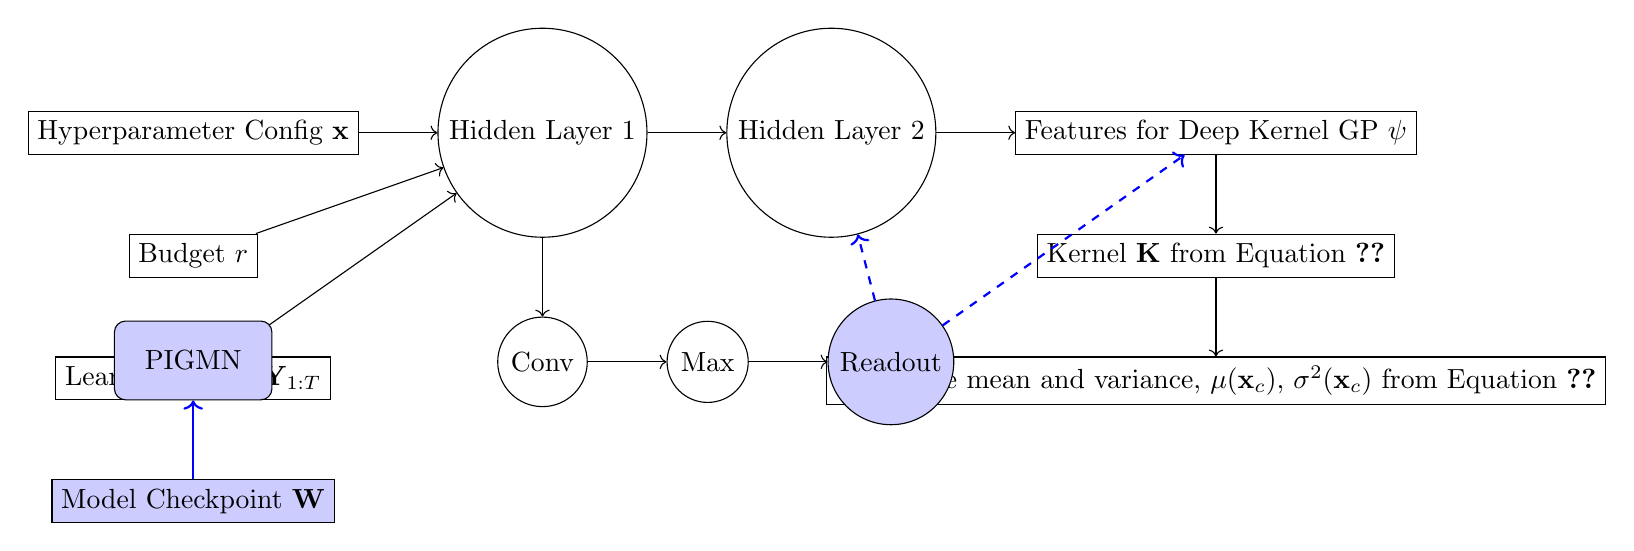
\begin{tikzpicture}[node distance=1cm, auto]
        % Nodes
        \node[draw, rectangle] (config) {Hyperparameter Config $\mathbf{x}$};
        \node[draw, rectangle, below=of config] (budget) {Budget $r$};
        \node[draw, rectangle, below=of budget] (learning_curve) {Learning Curve $\mathbf{Y}_{1:T}$};
        \node[draw, rectangle, below=of learning_curve, fill=blue!20] (checkpoint) {Model Checkpoint $\mathbf{W}$};
        \node[draw, circle, right=of config] (hidden_layer_1) {Hidden Layer 1};
        \node[draw, circle, right=of hidden_layer_1] (hidden_layer_2) {Hidden Layer 2};
        \node[draw, rectangle, right=of hidden_layer_2] (features) {Features for Deep Kernel GP $\psi$};
        \node[draw, rectangle, below=of features] (kernel) {Kernel $\mathbf{K}$ from Equation~\ref{eq:weight_kernel}};
        \node[draw, rectangle, below=of kernel] (output) {Predictive mean and variance, $\mu(\mathbf{x}_c)$, $\sigma^2(\mathbf{x}_c)$ from Equation~\ref{eq:weight_kernel}};
        
        % Arrows
        \draw[->] (config) -- (hidden_layer_1);
        \draw[->] (budget) -- (hidden_layer_1);
        \draw[->] (learning_curve) -- (hidden_layer_1);
        \draw[->] (hidden_layer_1) -- (hidden_layer_2);
        \draw[->] (hidden_layer_2) -- (features);
        \draw[->] (features) -- (kernel);
        \draw[->] (kernel) -- (output);
        
        % Additional nodes and arrows
        \node[draw, circle, below=of hidden_layer_1] (conv) {Conv};
        \node[draw, circle, right=of conv] (max_pool) {Max};
        \node[draw, circle, right=of max_pool, fill=blue!20] (readout) {Readout};
        
        \draw[->] (hidden_layer_1) -- (conv);
        \draw[->] (conv) -- (max_pool);
        \draw[->] (max_pool) -- (readout);
        
        \draw[->, blue, dashed, thick] (readout) -- (hidden_layer_2);
        \draw[->, blue, dashed, thick] (readout) -- (features);
        
        % Blue box around PIGMN
        \node[draw, rectangle, rounded corners, fill=blue!20, minimum width=2cm, minimum height=1cm, above=of checkpoint, anchor=south] (pigmn) {PIGMN};
        \draw[->, blue, thick] (checkpoint) -- (pigmn);
    \end{tikzpicture}
    \caption{We show an overview of our method, Forecasting Model Search (FMS), which builds on DyHPO's multifidelity method from Algorithm~\ref{alg:dyhpo}. Novel components of FMS are highlighted in \textcolor{blue}{blue} and further detailed in Algorithm~\ref{alg:fms}. We include DyHPO's features from the hyperparameter configuration, budget, and learning curve \cite{wistuba2023supervising}. Notably, we also featurize the model's checkpointed weights $\mathbf{W}$ with a permutation-invariant graph metanetwork (PIGMN) as in Section~\ref{pigms} for input to a deep kernel GP (see Equation~\ref{deepkernelgp}/\ref{eq:weight_kernel}). This provides the HPO with an -- often pre-existing -- rich source of information, which implicitly includes the architecture, dataset, loss, and optimization process. FMS shows improved predictions about hyperparameter performance across compute budgets (see Table~\ref{ktau-values}), improved quality of the final selected configuration across compute budgets (see Figure~\ref{fig:regret_over_time}), and a potential to generalize beyond what was seen in training (see Figure~\ref{fig:fms-transfer}). Specific design choices for this surrogate model are detailed in Appendix Section~\ref{meta-hyperparams}.}
    \label{fig:fms-diagram}
\end{figure}

\end{document}